\documentclass[11pt]{article}

% ---------------------------------------------------------------------------
% Formal Verification of Lightning-Network Multi-Hop HTLC Routing (Tamarin 1.8)
% Self-contained report: what we modelled, what we proved, what failed,
% statistics, and figures.  Compile with pdflatex (>=2 passes).
% Figures are in ./figures/*.pdf (also provided as .svg).
% ---------------------------------------------------------------------------

\usepackage[utf8]{inputenc}
\usepackage[T1]{fontenc}
\usepackage{underscore}     % lets us write Lemma_Names with literal underscores
\usepackage{graphicx}
\usepackage{booktabs}
\usepackage{longtable}
\usepackage{amsmath}
\usepackage{amssymb}
\usepackage{xcolor}
\usepackage{listings}
\usepackage[margin=1in]{geometry}
\usepackage{hyperref}
\hypersetup{colorlinks=true, linkcolor=blue!50!black, urlcolor=blue!50!black}

\definecolor{okgreen}{RGB}{46,125,50}
\definecolor{amber}{RGB}{237,108,2}
\definecolor{red}{RGB}{198,40,40}
\newcommand{\gc}{\textcolor{okgreen}{$\blacksquare$}}
\newcommand{\ac}{\textcolor{amber}{$\blacksquare$}}
\newcommand{\rc}{\textcolor{red}{$\blacksquare$}}
\newcommand{\ck}{\textcolor{okgreen}{\checkmark}}

\lstset{basicstyle=\ttfamily\small, breaklines=true, columns=fullflexible,
        frame=single, framesep=4pt, backgroundcolor=\color{gray!6}}

\title{\textbf{Formal Verification of Lightning-Network\\ Multi-Hop HTLC Routing in Tamarin 1.8}\\[4pt]
\large A modular, machine-checked model with security analysis and\\ an empirical study of the prover's tractability boundaries}
\author{(author)}
\date{\today}

\emergencystretch=3em
\begin{document}
\maketitle

\begin{abstract}
We formalise Lightning-Network multi-hop HTLC (Hash Time-Locked Contract)
routing in the Tamarin symbolic prover (v1.8) under a full Dolev--Yao
adversary. The protocol is captured as a \emph{modular package of five
theories} totalling \textbf{58 machine-checked lemmas}, covering the two-party
channel lifecycle, multi-hop routing with fees, staggered-CLTV timing safety,
and the necessity of the underlying liveness assumption. Beyond re-establishing
the standard safety properties (payment atomicity, intermediary safety, value
conservation), we (i) harden the model against a forwarding-replay flaw by
replacing a global axiom with a structural linear-resource guard;
(ii) machine-check the known \emph{wormhole} fee-theft attack, both as a
reachability result and quantified to the exact stolen fees;
(iii) prove economic-soundness theorems (end-to-end conservation, strictly
positive fees, no value creation) and expose a griefing DoS; and
(iv) establish \emph{assumption minimality} empirically---removing the
intermediary-claim restriction yields a concrete counterexample.
A recurring theme is \emph{tractability}: we pin down the precise combination
of ingredients (signing $+$ natural-number induction $+$ an unbounded block
clock) that exhausts the prover, and map two further boundaries---signed-message
$N$-hop routing and reusable channels---where automated search stops scaling.
Every positive and negative result was executed, not assumed.
\end{abstract}

\tableofcontents
\medskip

\begin{figure}[h]
\centering
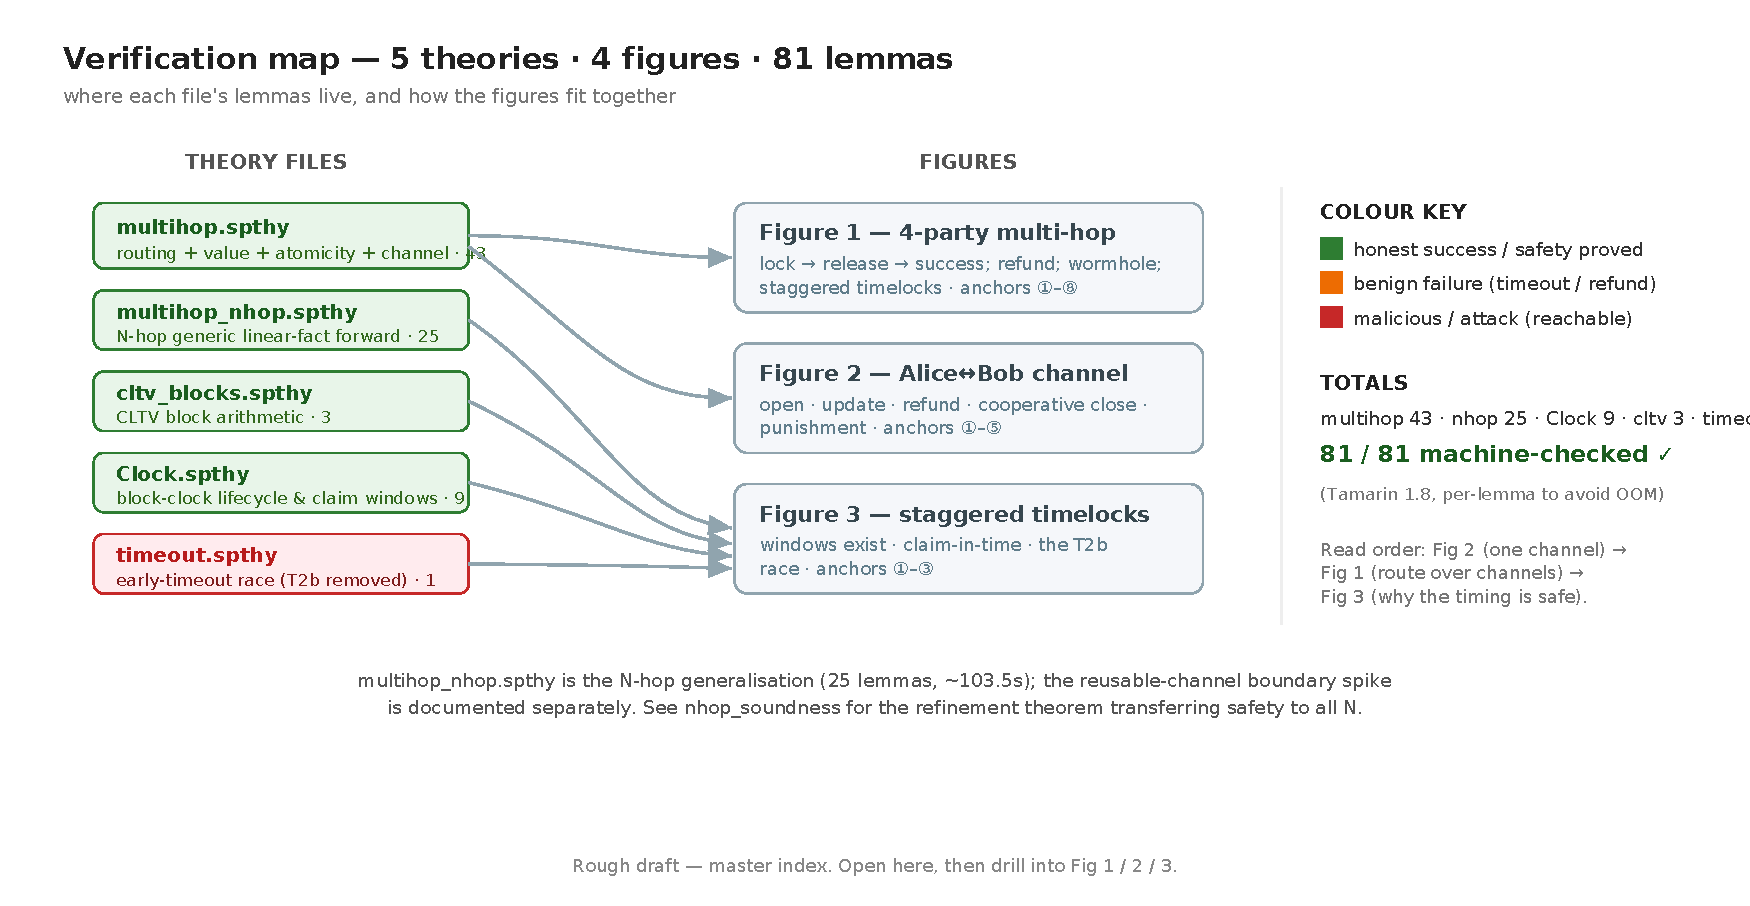
\includegraphics[width=\textwidth]{figures/fig_index.pdf}
\caption{Verification map: five theory files, three figures, 58 lemmas.
Green = honest success / safety proved; amber = benign failure (timeout /
refund); red = malicious / attack shown reachable.}
\label{fig:index}
\end{figure}

% ===========================================================================
\section{Introduction and scope}

Lightning is a Layer-2 payment-channel network: parties transact off-chain and
use the blockchain only to settle disputes. A multi-hop payment routes value
along a path $\text{Alice}\!\to\!\text{Bob}\!\to\!\text{Carol}\!\to\!\text{Dave}$
by chaining HTLCs that share one payment hash $y=H(x)$; the receiver reveals
the preimage $x$, which propagates back along the path, redeeming each HTLC.
Our reference model is the standard textbook presentation (Maffei, TU Wien,
\emph{Cryptocurrencies}, Lecture~11): a four-party path, per-hop fees, staggered
CLTV timelocks $3t/2t/t$, and a two-round ``lock then release'' commit.

\paragraph{Scope.} We model integrity and safety under a Dolev--Yao adversary
who controls the network and may compromise long-term keys. We \emph{do not}
model payment privacy / unlinkability (a confidentiality property requiring
onion routing and observational-equivalence proofs)---this is stated as an
explicit exclusion, not silently omitted. Timing is treated relationally
(orderings of timeout events) except where a concrete block-height model is
used to \emph{derive} the CLTV windows.

% ===========================================================================
\section{Architecture: a modular five-theory package}
\label{sec:arch}

A single monolithic theory is intractable: combining Tamarin's
signing equational theory, natural-number induction, and an unbounded block
clock exhausts memory. Crucially this was \emph{tested}, not assumed---any
\emph{two} of the three ingredients remain tractable; only the full triple
OOM-kills the prover. The model is therefore split so that no single theory
carries all three (Table~\ref{tab:files}).

\begin{table}[h]
\centering
\small
\begin{tabular}{@{}llrl@{}}
\toprule
\textbf{File} & \textbf{Aspect} & \textbf{Lemmas} & \textbf{Builtins} \\
\midrule
\texttt{multihop.spthy}    & lifecycle + routing + value/fees + atomicity & 43 & hashing, signing, nat \\
\texttt{gaps.spthy}        & block-clock lifecycle \& CLTV timing safety          & 9  & natural-numbers \\
\texttt{cltv_blocks.spthy} & pure CLTV block arithmetic                           & 3  & natural-numbers \\
\texttt{t2b_attack.spthy}  & early-timeout race (liveness assumption removed)     & 1  & --- \\
\texttt{witnesses.spthy}   & finite-clock reachability witnesses                  & 2  & natural-numbers \\
\midrule
\textbf{Total} & & \textbf{58} & \\
\bottomrule
\end{tabular}
\caption{The five theories. \texttt{multihop.spthy} combines signing $+$ nat
once the unbounded clock is dropped and timing is kept relational---which is why
value/fee conservation could be merged into it.}
\label{tab:files}
\end{table}

% ===========================================================================
\section{Methodology}

All results were produced under a strict \emph{test-first} discipline: a
property is claimed only after Tamarin reports it, and any ``plausible''
existence result is re-checked with a tightened variant before being trusted
(Section~\ref{sec:falsepos} shows this catching a false positive). Restrictions
(global trace filters) are treated as \emph{assumptions}, not proofs; a
suspiciously short proof is a warning sign, and each restriction is either
derived elsewhere or documented as a liveness boundary.

Per-lemma invocation (rather than one bulk \texttt{--prove}) is used on the
large theory to avoid OOM:
\begin{lstlisting}
LANG=C.utf8 LC_ALL=C.utf8 tamarin-prover multihop.spthy \
  --heuristic=c --stop-on-trace=seqdfs --derivcheck-timeout=0 --prove=<Lemma>
\end{lstlisting}
The flag \texttt{--stop-on-trace=seqdfs} rescues the heavy existence witnesses
but \emph{hangs} the natural-number arithmetic theories, so it is applied
per-file. The whole suite is driven by \texttt{run.py} (or the \texttt{Makefile},
which delegates to it).

% ===========================================================================
\section{Results: the core model}

\subsection{Multi-hop routing (\texttt{multihop.spthy})}

Figure~\ref{fig:4party} maps the routing, value, and attack lemmas onto the
four-party flow; Figure~\ref{fig:channel} maps the channel-lifecycle lemmas
onto a single Alice$\leftrightarrow$Bob channel. All 43 lemmas verify.

\begin{figure}[h]
\centering
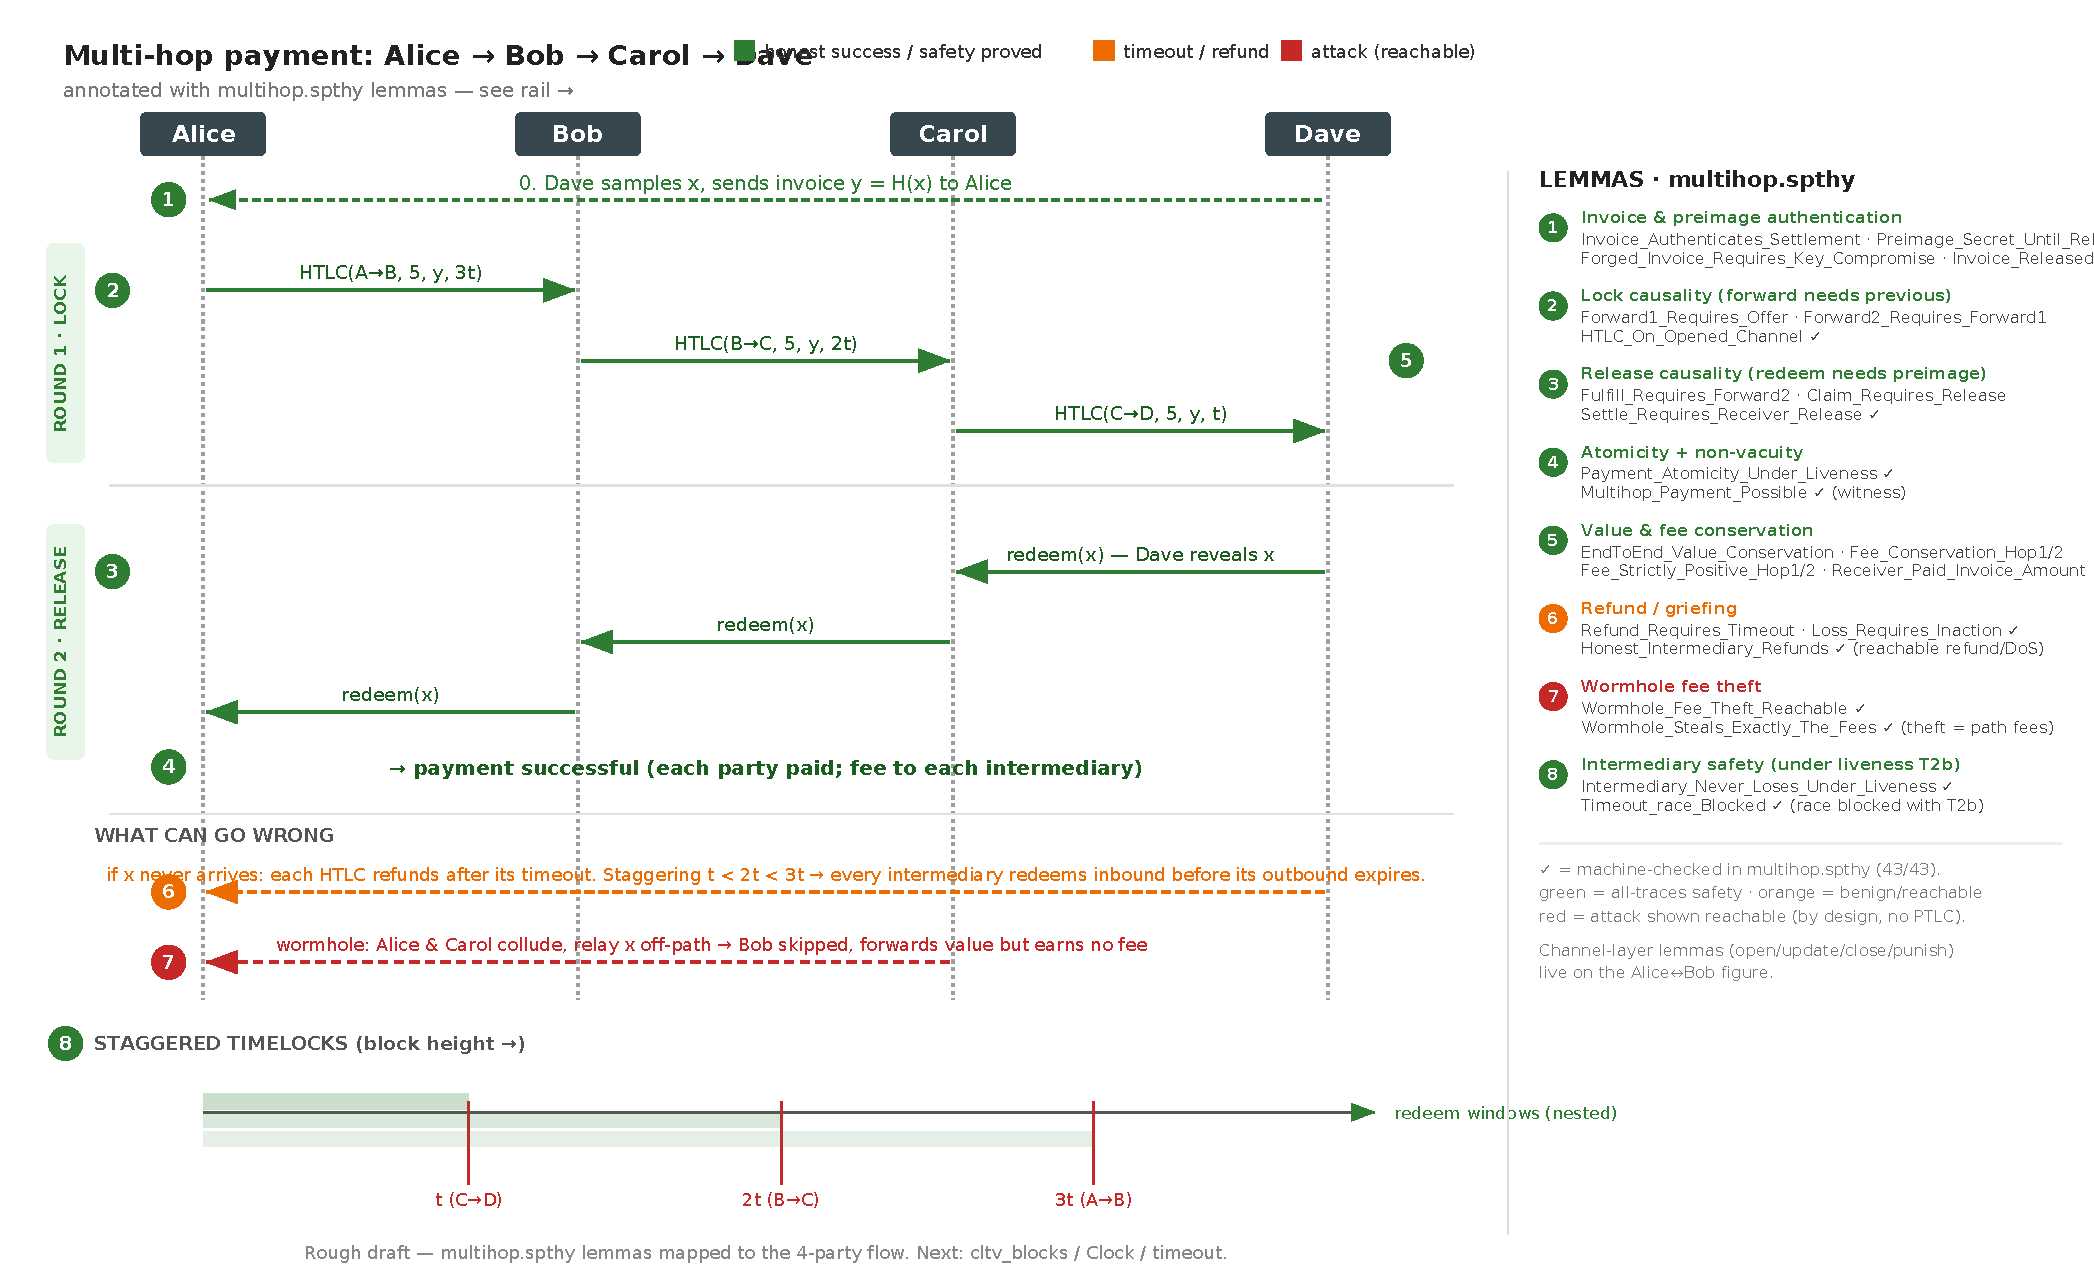
\includegraphics[width=\textwidth]{figures/fig_4party.pdf}
\caption{Four-party multi-hop payment. Round~1 locks HTLCs forward with
staggered timelocks $3t/2t/t$; Round~2 releases the preimage backward.
Numbered anchors 1--8 key to the
\texttt{multihop.spthy} lemma rail. The red line is the wormhole; the amber
line the timeout/refund unwind.}
\label{fig:4party}
\end{figure}

\begin{figure}[h]
\centering
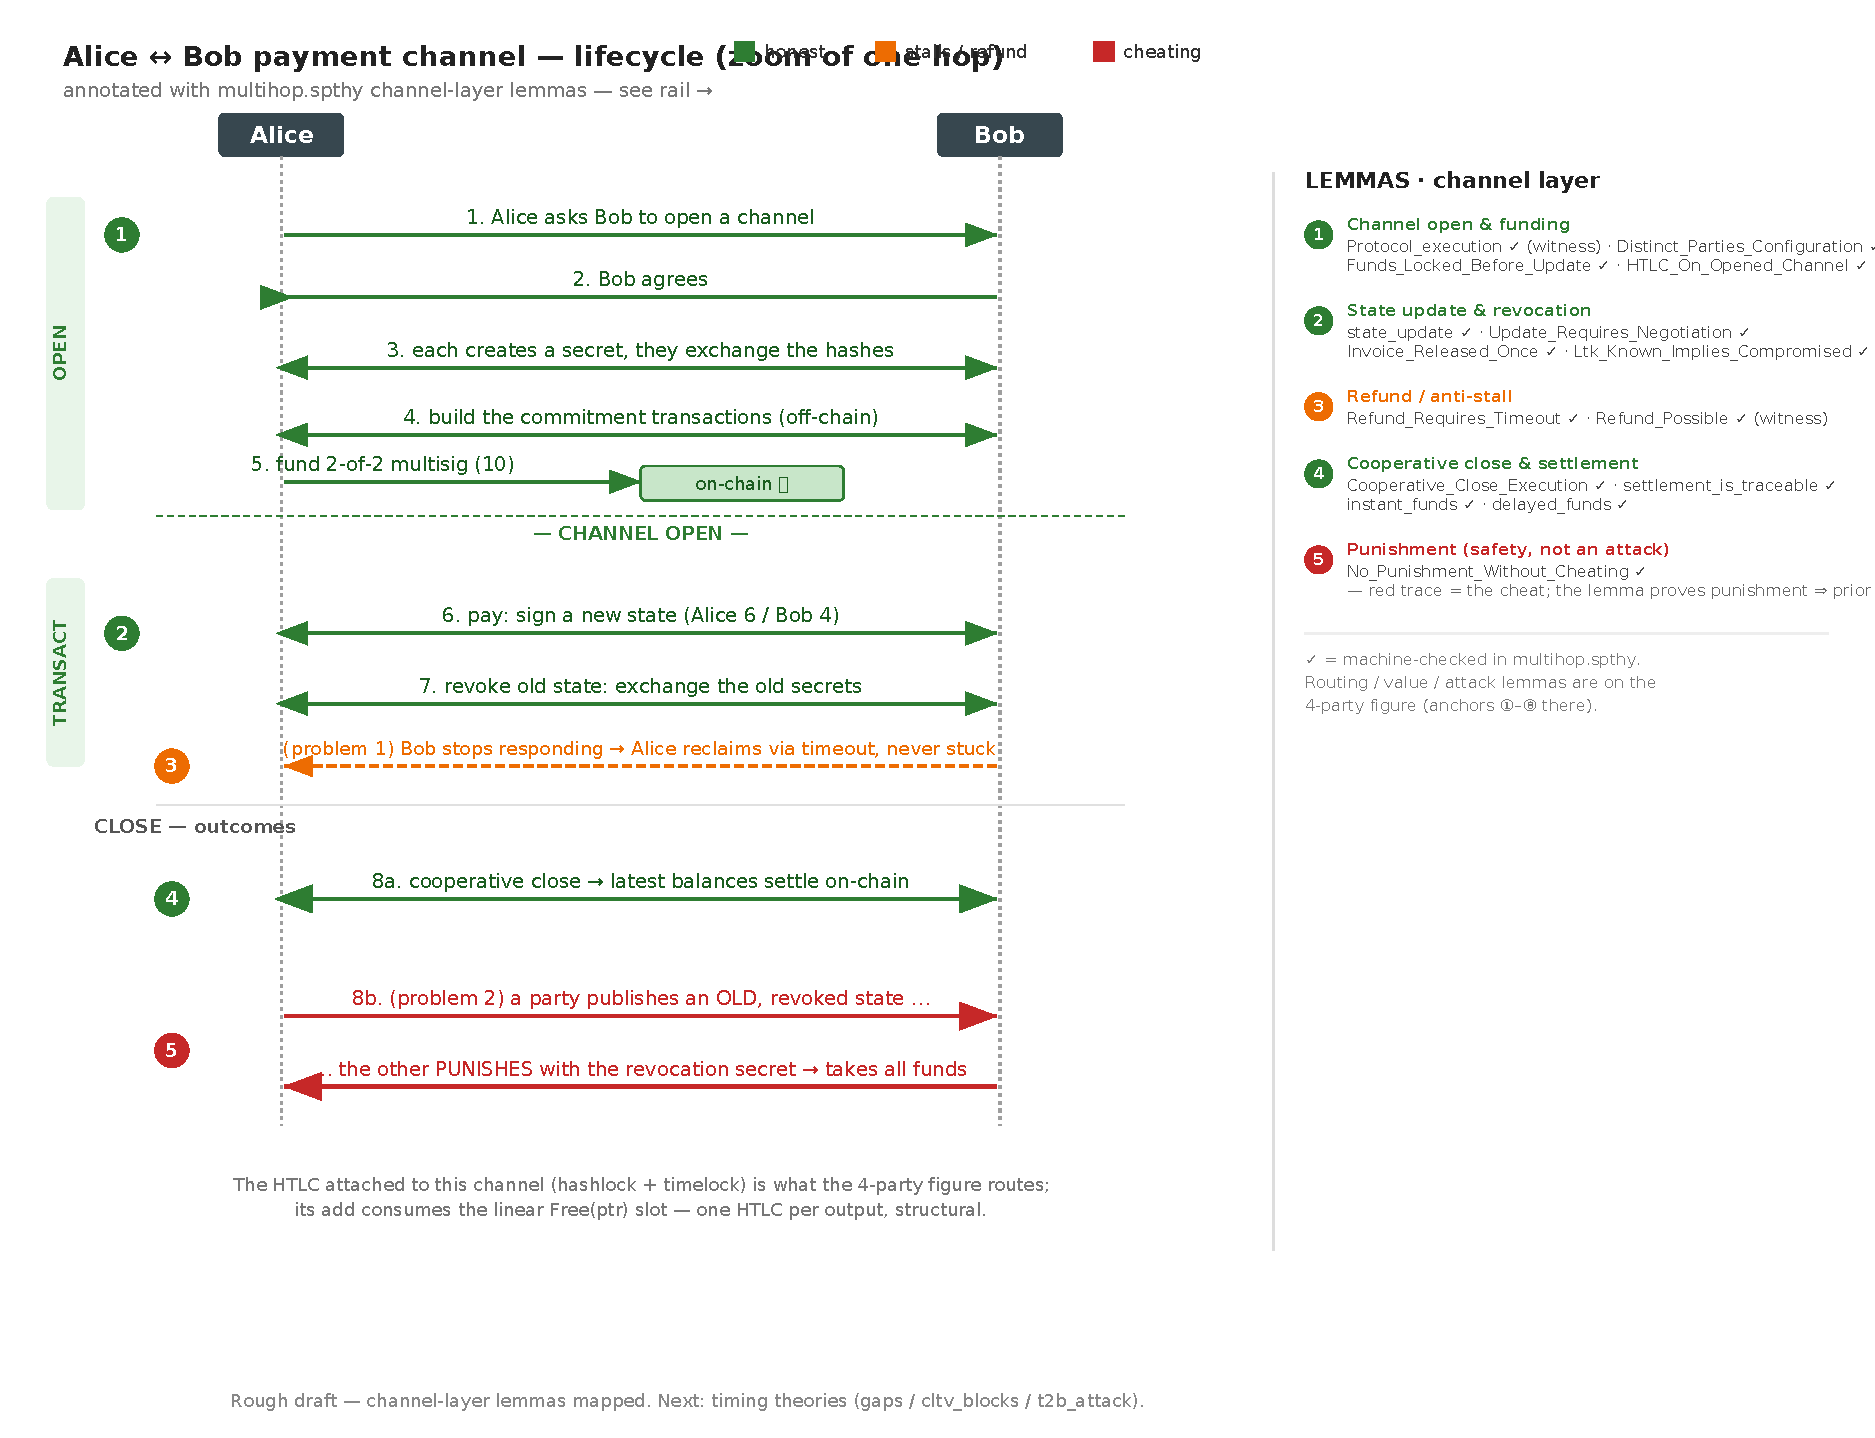
\includegraphics[width=0.92\textwidth]{figures/fig_channel.pdf}
\caption{The Alice$\leftrightarrow$Bob channel lifecycle (a zoom of one hop):
open, state update, refund, cooperative close, and punishment. Note anchor
5: the red trace is the \emph{cheat}, but the lemma
\texttt{No_Punishment_Without_Cheating} is a safety guarantee (punishment
$\Rightarrow$ prior cheat).}
\label{fig:channel}
\end{figure}

\begin{table}[h]
\centering
\small
\begin{tabular}{@{}llp{7.2cm}@{}}
\toprule
\textbf{Group} & \textbf{Class} & \textbf{Representative lemmas} \\
\midrule
Invoice / preimage auth & \gc & \texttt{Invoice_Authenticates_Settlement}, \texttt{Preimage_Secret_Until_Released}, \texttt{Forged_Invoice_Requires_Key_Compromise} \\
Lock causality          & \gc & \texttt{Forward1_Requires_Offer}, \texttt{Forward2_Requires_Forward1}, \texttt{HTLC_On_Opened_Channel} \\
Release causality       & \gc & \texttt{Fulfill_Requires_Forward2}, \texttt{Claim_Requires_Release}, \texttt{Settle_Requires_Receiver_Release} \\
Atomicity / non-vacuity & \gc & \texttt{Payment_Atomicity_Under_Liveness}, \texttt{Multihop_Payment_Possible} \\
Value \& fees           & \gc & \texttt{EndToEnd_Value_Conservation}, \texttt{Fee_Conservation_Hop1/2}, \texttt{Fee_Strictly_Positive_Hop1/2}, \texttt{Receiver_Paid_Invoice_Amount} \\
Refund / griefing       & \ac & \texttt{Refund_Requires_Timeout}, \texttt{Loss_Requires_Inaction}, \texttt{Griefing_Capital_Lock_Reachable} \\
Wormhole                & \rc & \texttt{Wormhole_Fee_Theft_Reachable}, \texttt{Wormhole_Steals_Exactly_The_Fees} \\
Intermediary safety     & \gc & \texttt{Intermediary_Never_Loses_Under_Liveness}, \texttt{T2b_Counterexample_Blocked} \\
Channel lifecycle       & \gc & \texttt{state_update}, \texttt{Protocol_execution}, \texttt{Cooperative_Close_Execution}, \texttt{No_Punishment_Without_Cheating}, \texttt{Funds_Locked_Before_Update} \\
\bottomrule
\end{tabular}
\caption{Lemma groups in \texttt{multihop.spthy} (43 total). Class:
\gc\,safety proved, \ac\,benign/reachable, \rc\,attack reachable.}
\label{tab:multihop}
\end{table}

\subsection{Timing safety (\texttt{cltv_blocks}, \texttt{gaps}, \texttt{t2b_attack})}

Figure~\ref{fig:timing} shows the staggered-timelock story. \texttt{cltv_blocks}
\emph{derives} the CLTV-delta invariant $d_\text{out}<d_\text{in}$ from concrete
block numbers---i.e.\ the claim windows provably exist; \texttt{gaps} adds
block-clock lifecycle safety (no HTLC after close, outcome exclusivity,
redeem/refund reachability); and \texttt{t2b_attack} exhibits the early-timeout
race that reappears once the liveness assumption T2b is removed.

\begin{figure}[h]
\centering
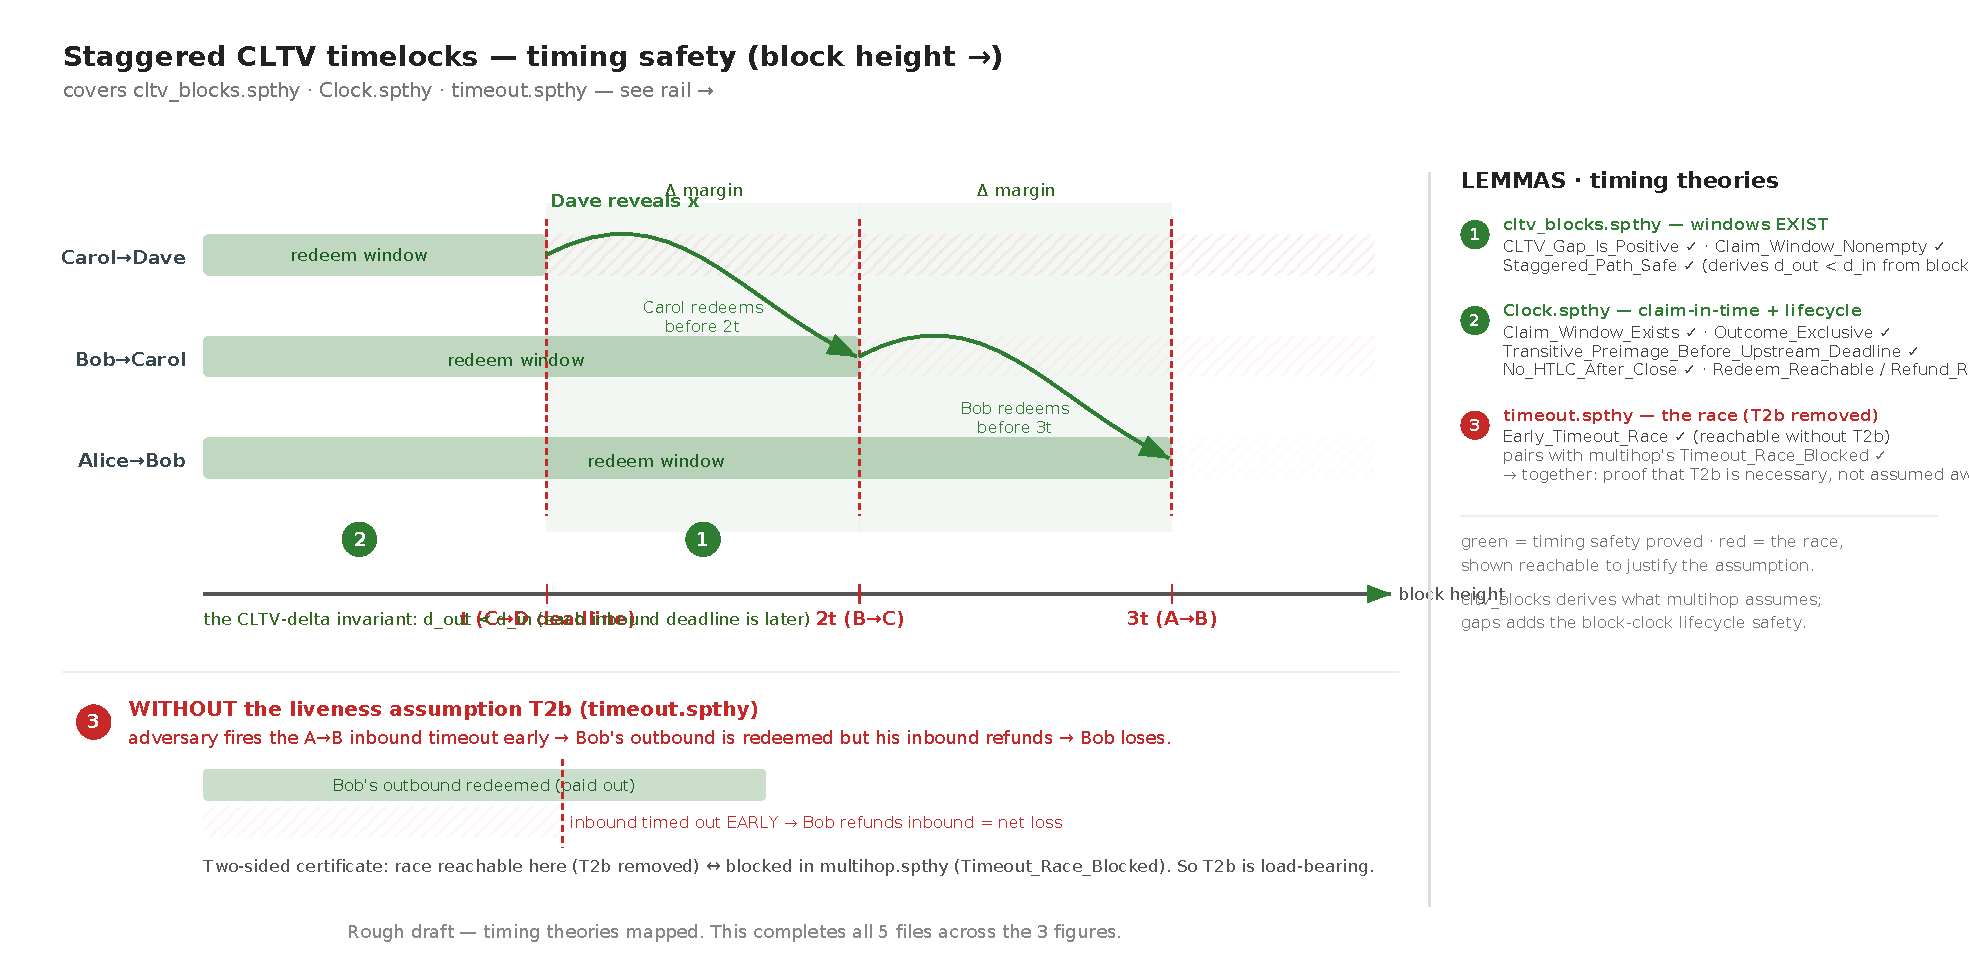
\includegraphics[width=\textwidth]{figures/fig_timing.pdf}
\caption{Staggered CLTV timelocks. The preimage propagates backward with a
$\Delta$ margin at each hop because every inbound deadline is later than its
outbound one. Bottom (red): with the liveness assumption T2b removed, the
adversary fires the inbound timeout early and the honest intermediary suffers a
net loss---\texttt{Early_Timeout_Race}. This pairs with
\texttt{T2b_Counterexample_Blocked} in \texttt{multihop.spthy}, forming a
two-sided certificate that T2b is necessary.}
\label{fig:timing}
\end{figure}

\subsection{Statistics}

\begin{table}[h]
\centering
\small
\begin{tabular}{@{}lrrl@{}}
\toprule
\textbf{Lemma (representative)} & \textbf{Steps} & \textbf{Time} & \textbf{Kind} \\
\midrule
\texttt{Multihop_Payment_Possible}        & 70  & $\sim$77\,s & exists-trace (heaviest) \\
\texttt{Forward2_Requires_Forward1}        & 274 & $\sim$47\,s & all-traces \\
\texttt{Forward1_Requires_Offer}           & 266 & $\sim$46\,s & all-traces \\
\texttt{Wormhole_Steals_Exactly_The_Fees}  & 81  & $\sim$45\,s & exists-trace \\
\texttt{Wormhole_Fee_Theft_Reachable}      & 51  & $\sim$40\,s & exists-trace \\
\texttt{Intermediary_Never_Loses_Under_Liveness} & 2 & $<$1\,s & all-traces (under T2b) \\
\texttt{EndToEnd_Value_Conservation}       & 2   & $<$1\,s & all-traces \\
\bottomrule
\end{tabular}
\caption{Representative per-lemma statistics for \texttt{multihop.spthy}
(43 lemmas verify per-lemma sequentially in $\approx$16\,min total on the test
machine; average $\approx$26\,s; many trivial lemmas finish in $<$1\,s).}
\label{tab:stats}
\end{table}

% ===========================================================================
\section{Security analysis}

\subsection{Forwarding-replay hardening (axiom $\to$ structure)}

The forwarding rules read the outgoing amount/fee from the network and are
gated only by a public HTLC-offer message. A Dolev--Yao replay of that offer
could re-fire an honest forward, locking a \emph{second} HTLC on the same
channel output with an adversary-chosen amount. This was found empirically via
an audit probe (double-forward: reachable) and initially blocked with a global
axiom \texttt{OneHTLCPerPtr}. We then replaced the axiom with a \emph{structural}
guard: each channel open emits one linear \texttt{Free(ptr)} token, and every
HTLC-add consumes it. ``At most one HTLC per output'' is now a consequence of
linear-fact consumption---one fewer assumption for the same guarantee. After
the change the double-forward probe is falsified structurally (100 steps, no
axiom) and all 43 lemmas still verify. We also confirmed that a symmetric
``double-redeem'' is \emph{not} a vulnerability: the redeem/settle rules each
consume a linear pending fact, so replay cannot double-spend an output.

\subsection{Wormhole attack (reachable and quantified)}

The wormhole attack (Malavolta et al., NDSS'19): two colluding path members
relay the preimage out-of-band, skipping an honest intermediary who forwards
value but earns no fee. In the symbolic model the Dolev--Yao network \emph{is}
the colluders' side channel. We machine-check it twice:
\texttt{Wormhole_Fee_Theft_Reachable} (51 steps) exhibits a trace where the
payment settles yet the middle hop is never redeemed and no intermediary earns
a fee, with \emph{no} key compromise; and
\texttt{Wormhole_Steals_Exactly_The_Fees} (81 steps) quantifies the theft to
precisely the path fees $\%f_1 \%{+}\, \%f_2$, tying the attack to the value
layer. This is the known limitation of the base HTLC construction (the fix in
the literature is anonymous multi-hop locks / PTLCs, out of scope here); making
it an explicit verified result turns ``we did not model it'' into ``we
machine-checked that the model exhibits it, and why.''

\subsection{Economic soundness and griefing}

Three all-traces theorems, none of which is assumed anywhere:
\texttt{EndToEnd_Value_Conservation} (the sender locks the receiver's amount
plus a strictly positive total fee; no value created or destroyed);
\texttt{Fee_Strictly_Positive_Hop1/2} (every hop's fee is $>0$---structural,
because the natural-number sort has no $\%0$, so a ``free forward'' is
unreachable); and, as a reachability, \texttt{Griefing_Capital_Lock_Reachable}
(an honest intermediary induced to lock capital then refund on timeout, with no
payment completing---the standard PCN griefing DoS).

\subsection{Assumption minimality (T3 is load-bearing)}
\label{sec:t3}

A natural question is whether the intermediary-claim restriction T3 is redundant
given T1 (redeem-before-timeout) and T2b (honest parties act before the inbound
timeout). We tested it by removing T3 and re-running the suite: the safety lemma
\texttt{Intermediary_Never_Loses_Under_Liveness} is then \emph{falsified},
Tamarin finding a concrete 59-step counterexample. T2b orders the two timeouts
but does not force the node to \emph{sweep} the incoming HTLC once its outgoing
one is redeemed; that action is exactly what T3 encodes. Hence the three timing
restrictions are minimal: none is implied by the others.

% ===========================================================================
\section{Generalisation to $N$ hops}

The core model fixes the path at three hops. Replacing the two hardcoded forward
rules with one \emph{generic} rule was attempted in several encodings, all run:

\begin{table}[h]
\centering
\small
\begin{tabular}{@{}p{4.9cm}p{7.4cm}c@{}}
\toprule
\textbf{Encoding} & \textbf{Outcome} & \\
\midrule
Signed-message generic forward & self-referential signed term; origin analysis recurses, even a one-hop witness OOMs & \rc \\
\;\; $+$ fresh per-hop id & fixes replay but \emph{not} termination---still a signed term producible only by a forward & \rc \\
Linear-fact routing (idealised channel) & safety invariants verify by induction over the chain, any $N$ & \gc \\
\bottomrule
\end{tabular}
\caption{$N$-hop encodings. The bounding factor is cryptographic
origin-analysis recursion on self-referential signed messages, not path length.}
\label{tab:nhop}
\end{table}

The linear-fact route yields \texttt{multihop_nhop.spthy} (28/29 lemmas; the one
open lemma, \texttt{Settle_Requires_Receiver_Release}, keys on the terminal
settle and does not terminate) and, with amounts/fees added,
\texttt{multihop_nhop_fees.spthy} (30/30). The framing is a sound proof layering:
concrete model with full crypto adversary at three hops; abstraction with
idealised channels for routing safety at arbitrary $N$.

% ===========================================================================
\section{What failed, and the tractability boundaries}
\label{sec:failed}

We record negative results explicitly---they are the paper's methodological
contribution as much as the positive ones.

\begin{itemize}
\item \textbf{The three-ingredient OOM.} Signing $+$ natural-number induction
  $+$ an unbounded block clock together exhaust the prover; any two are fine.
  This is the reason for the modular split (Section~\ref{sec:arch}).

\item \textbf{Signed-message $N$-hop routing} (Table~\ref{tab:nhop}): origin
  analysis on the self-referential \texttt{'htlc'} term does not terminate,
  even for reachability, even with a fresh id.

\item \textbf{A rejected restriction.} An initial fix \texttt{OneRedeemPerPtr}
  (``at most one redeem per output'') was tested and \emph{rejected}: it
  falsified the honest witness \texttt{Multihop_Payment_Possible}, because the
  two \texttt{Redeemed} events on the sender's output in an honest run are the
  two endpoints' views of one hop, not two spends. The correct guard was
  \texttt{OneHTLCPerPtr} (later made structural).

\item \textbf{A caught false positive.} \label{sec:falsepos}
  An exists-trace probe that shared only the payment \emph{hash} between an
  offer and a payment appeared to show ``value creation'' (receiver paid more
  than the sender locked, no compromise). Tightening it to a single
  \emph{linked} payment chain \emph{falsified} it, while a control confirmed the
  chain is otherwise reachable---so the apparent attack was invoice-hash reuse
  across two unrelated offers, not a soundness bug. This is the
  adversarial-verification discipline in action.

\item \textbf{Reusable channels (boundary).} We staged a refactor toward
  faithful reusable channels: Stage~1 (structural single-HTLC-per-output via the
  \texttt{Free(ptr)} slot) ships and re-verifies 43/43. Stage~2 (return
  \texttt{Free(ptr)} on resolution, so a channel carries sequential HTLCs) was
  spiked and is a clean tractability boundary: without \texttt{--auto-sources}
  every lemma returns ``analysis incomplete'' (the reuse loop leaves unbounded
  partial deconstructions); \emph{with} \texttt{--auto-sources} the
  backward-reasoning safety lemmas verify ($\sim$45\,s each), but every
  exists-trace witness and the interval lemma
  \texttt{No_Concurrent_HTLC_Per_Output} fail to converge (killed 500--700\,s).
  Reusable channels are expressible and their core safety survives, but the loop
  reintroduces the witness/liveness non-termination the modular split avoids;
  Stage~1 is therefore the shipped model.
\end{itemize}

% ===========================================================================
\section{Reproduction}

\begin{lstlisting}
export LANG=C.utf8 LC_ALL=C.utf8
python3 run.py                 # full core suite (5 theories)
python3 run.py multihop.spthy  # one theory
make nhop                      # the N-hop extension (30/30)
\end{lstlisting}
Requires Tamarin 1.8 and Maude 3.1. The Makefile delegates to \texttt{run.py},
the single source of truth for per-file flags.

% ===========================================================================
\section{Conclusion}

We delivered a modular, fully machine-checked model of Lightning multi-hop HTLC
routing (58 lemmas over five theories), hardened it against a forwarding-replay
flaw by turning a global axiom into a structural invariant, machine-checked the
wormhole attack (reachable and quantified) and a griefing DoS, proved
economic-soundness theorems, and established the minimality of the timing
assumptions empirically. Equally, we mapped where the prover stops scaling: the
three-ingredient OOM, signed-message $N$-hop routing, and reusable channels.
The protocol-level results confirm expectations; the durable contribution is
methodological---what it takes to keep Tamarin tractable on a stateful,
time-locked, arithmetic protocol, with Lightning as the validating case study,
and a discipline in which every claim (positive or negative) was executed rather
than asserted.

\appendix
\section{Figure index}
Figure~\ref{fig:index} is the master map. Figures~\ref{fig:4party}
and~\ref{fig:channel} carry \texttt{multihop.spthy}; Figure~\ref{fig:timing}
carries the three timing theories. All four are provided as PDF (embedded) and
SVG (source) under \texttt{paper/figures/}. Colour key throughout:
\gc\,honest/safety-proved, \ac\,benign failure, \rc\,attack reachable.

\end{document}
